%% no need for  \DeclareGraphicsExtensions{.pdf,.eps}

\documentclass[12pt,letterpaper,english]{article}
\usepackage{times}
\usepackage[T1]{fontenc}
\IfFileExists{url.sty}{\usepackage{url}}
                      {\newcommand{\url}{\texttt}}

\usepackage{babel}
%\usepackage{noweb}
\usepackage{Rd}

\usepackage{Sweave}

%\VignetteIndexEntry{Performance Attribution from Bacon}
%\VignetteDepends{PerformanceAnalytics}
%\VignetteKeywords{returns, performance, risk, benchmark, portfolio}
%\VignettePackage{PerformanceAnalytics}

%\documentclass[a4paper]{article}
%\usepackage[noae]{Sweave}
%\usepackage{ucs}
%\usepackage[utf8x]{inputenc}
%\usepackage{amsmath, amsthm, latexsym}
%\usepackage[top=3cm, bottom=3cm, left=2.5cm]{geometry}
%\usepackage{graphicx}
%\usepackage{graphicx, verbatim}
%\usepackage{ucs}
%\usepackage[utf8x]{inputenc}
%\usepackage{amsmath, amsthm, latexsym}
%\usepackage{graphicx}

\title{Commodity Index Fund Performance Analysis}
\author{Shubhankit Mohan}

\begin{document}
\Sconcordance{concordance:Managers.tex:Managers.Rnw:%
1 46 1 1 6 28 1 1 3 1 2 6 1 1 2 20 0 1 2 3 1 1 2 15 0 1 2 16 1 1 7 1 2 %
32 1 1 7 1 2 16 1 1 2 7 0 1 1 9 0 1 2 8 1 1 6 1 2 26 1 1 3 1 2 2 1 1 3 %
1 2 7 1 2 2 2 1}


\maketitle


\begin{abstract}
The fact that many hedge fund returns exhibit extraordinary levels of serial correlation is now well-known and generally accepted as fact. The effect of this autocorrelation on investment returns diminishes the apparent risk of such asset classes as the true returns/risk is easily \textbf{camouflaged} within a haze of liquidity, stale prices, averaged price quotes and smoothed return reporting. We highlight the effect \emph{autocorrelation} and \emph{drawdown} has on performance analysis by investigating the results of functions developed during the Google Summer of Code 2013 on \textbf{commodity based index} .
\end{abstract}

\tableofcontents



\section{Background}
The investigated fund index that tracks a basket of \emph{commodities} to measure their performance.The value of these indexes fluctuates based on their underlying commodities, and this value depends on the \emph{component}, \emph{methodology} and \emph{style} to cover commodity markets .

A brief overview of the indicies invested in our report are : 
  \begin{itemize}
    \item
     \textbf{DJUBS Commodity index} :  is a broadly diversified index that allows investors to track commodity futures through a single, simple measure. As the index has grown in popularity since its introduction in 1998, additional versions and a full complement of sub-indices have been introduced. Together, the family offers investors a comprehensive set of tools for measuring the commodity markets.
      \item
 \textbf{Morningstar CLS index} : is a simple rules-based trend following index operated in commodities
   \item
    \textbf{Newedge CTI} :  includes funds that utilize a variety of investment strategies to profit from price moves in commodity markets.
Managers typically use either (i) a trading orientated approach,involving the trading of physical commodity products and/or of commodity
derivative instruments in either directional or relative value strategies; Or (ii) Long short equity strategies focused on commodity related stocks.
  \end{itemize}
%Let $X \sim N(0,1)$ and $Y \sim \textrm{Exponential}(\mu)$.  Let
%$Z = \sin(X)$. $\sqrt{X}$.
  
%$\hat{\mu}$ = $\displaystyle\frac{22}{7}$
%e^{2 \mu} = 1
%\begin{equation}
%\left(\sum_{t=1}^{T} R_t/T\right) = \hat{\mu} \\
%\end{equation}

\section{Performance Summary Chart}

Given a series  of historical returns \((R_1,R_2, . . .,R_T)\) from \textbf{January-96} to \textbf{December-2006}, create a wealth index chart, bars for per-period performance, and underwater chart for drawdown of the 3 funds.

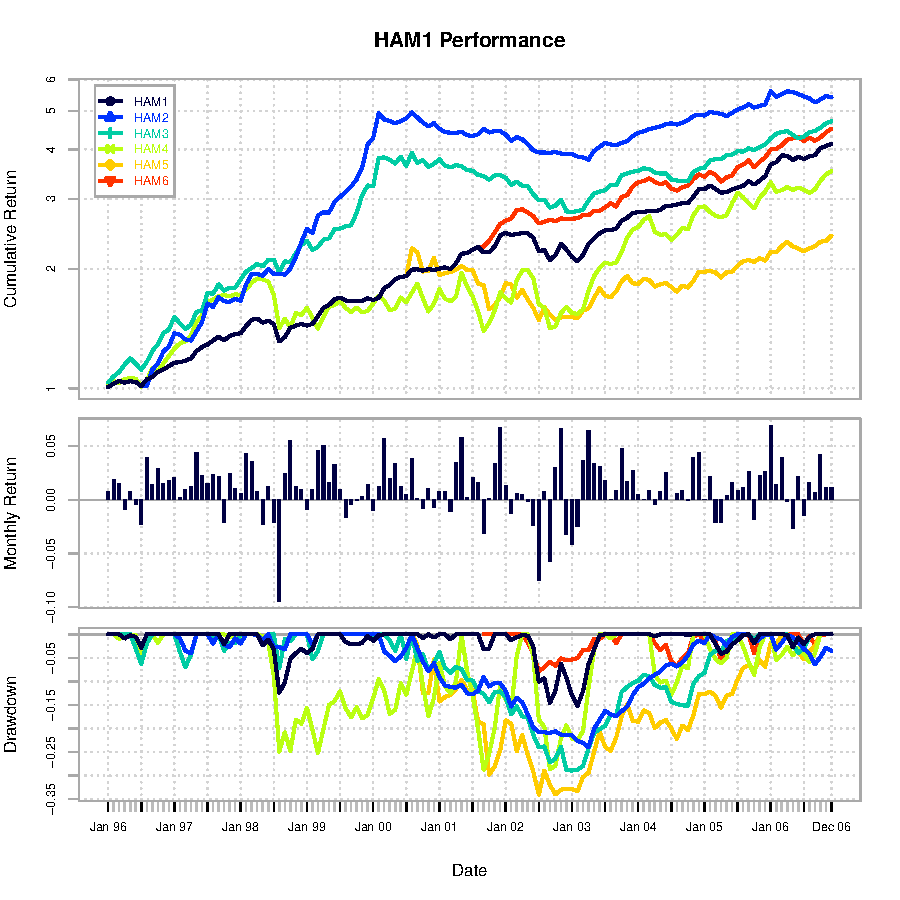
\includegraphics{Managers-002}

The above figure shows the behavior of the respective fund performance, which is \textbf{upward} trending for all the funds till the period of \textbf{"January-2008"}.For comparative purpose, one can observe the distinct \textbf{drawdown} of \textbf{Newedge CTI} since the latter period.

\section{Statistical and Drawdown Analysis}

A summary of Fund Return series characteristics show that \textbf{DJUBS.Commodity} performs worse relatively to it's peers.The most distinct characteristic being highest : \textbf{Variance, Stdev, SE Mean} and well as negative \textbf{Skewness} .The table shows clearly, that the returns of all the hedge fund indices are non-normal.Presence of \emph{negative} skewness is a major area of concern for the downside risk potential and expected maximum loss.

\begin{Schunk}
\begin{Soutput}
                    HAM1     HAM2     HAM3     HAM4    HAM5    HAM6
Observations    132.0000 125.0000 132.0000 132.0000 77.0000 64.0000
NAs               0.0000   7.0000   0.0000   0.0000 55.0000 68.0000
Minimum          -0.0944  -0.0371  -0.0718  -0.1759 -0.1320 -0.0404
Quartile 1        0.0000  -0.0098  -0.0054  -0.0198 -0.0164 -0.0016
Median            0.0112   0.0082   0.0102   0.0138  0.0038  0.0128
Arithmetic Mean   0.0111   0.0141   0.0124   0.0110  0.0041  0.0111
Geometric Mean    0.0108   0.0135   0.0118   0.0096  0.0031  0.0108
Quartile 3        0.0248   0.0252   0.0314   0.0460  0.0309  0.0255
Maximum           0.0692   0.1556   0.1796   0.1508  0.1747  0.0583
SE Mean           0.0022   0.0033   0.0032   0.0046  0.0052  0.0030
LCL Mean (0.95)   0.0067   0.0076   0.0062   0.0019 -0.0063  0.0051
UCL Mean (0.95)   0.0155   0.0206   0.0187   0.0202  0.0145  0.0170
Variance          0.0007   0.0013   0.0013   0.0028  0.0021  0.0006
Stdev             0.0256   0.0367   0.0365   0.0532  0.0457  0.0238
Skewness         -0.6588   1.4580   0.7908  -0.4311  0.0738 -0.2800
Kurtosis          2.3616   2.3794   2.6829   0.8632  2.3143 -0.3489
\end{Soutput}
\end{Schunk}


The results are consistent with Drawdown Analysis in which \textbf{DJUBS.Commodity} performs worse relatively to it's peers.

\begin{Schunk}
\begin{Soutput}
                                HAM1    HAM2    HAM3    HAM4    HAM5    HAM6
Semi Deviation                0.0191  0.0201  0.0237  0.0395  0.0324  0.0175
Gain Deviation                0.0169  0.0347  0.0290  0.0311  0.0313  0.0149
Loss Deviation                0.0211  0.0107  0.0191  0.0365  0.0324  0.0128
Downside Deviation (MAR=10%)  0.0178  0.0164  0.0214  0.0381  0.0347  0.0161
Downside Deviation (Rf=0%)    0.0145  0.0116  0.0174  0.0341  0.0304  0.0121
Downside Deviation (0%)       0.0145  0.0116  0.0174  0.0341  0.0304  0.0121
Maximum Drawdown              0.1518  0.2399  0.2894  0.2874  0.3405  0.0788
Historical VaR (95%)         -0.0258 -0.0294 -0.0425 -0.0799 -0.0733 -0.0341
Historical ES (95%)          -0.0513 -0.0331 -0.0555 -0.1122 -0.1023 -0.0392
Modified VaR (95%)           -0.0342 -0.0276 -0.0368 -0.0815 -0.0676 -0.0298
Modified ES (95%)            -0.0610 -0.0614 -0.0440 -0.1176 -0.0974 -0.0390
\end{Soutput}
\end{Schunk}
\section{Non-i.i.d GSoC Usage}
\subsection{Auctocorrelation Adjusted Standard Deviation}
Given a sample of historical returns \((R_1,R_2, . . .,R_T)\),the method assumes the fund manager smooths returns in the following manner, when 't' is the unit time interval, with  $\rho$\ as the respective term autocorrelation coefficient

%Let $X \sim N(0,1)$ and $Y \sim \textrm{Exponential}(\mu)$.  Let
%$Z = \sin(X)$. $\sqrt{X}$.
  
%$\hat{\mu}$ = $\displaystyle\frac{22}{7}$
%e^{2 \mu} = 1
%\begin{equation}
%\left(\sum_{t=1}^{T} R_t/T\right) = \hat{\mu} \\
%\end{equation}
\begin{equation}
 \sigma_{T}  =   \sqrt{  \sum_k^n(\sigma_{t}^2 +  2*\rho_i) } \\
\end{equation}


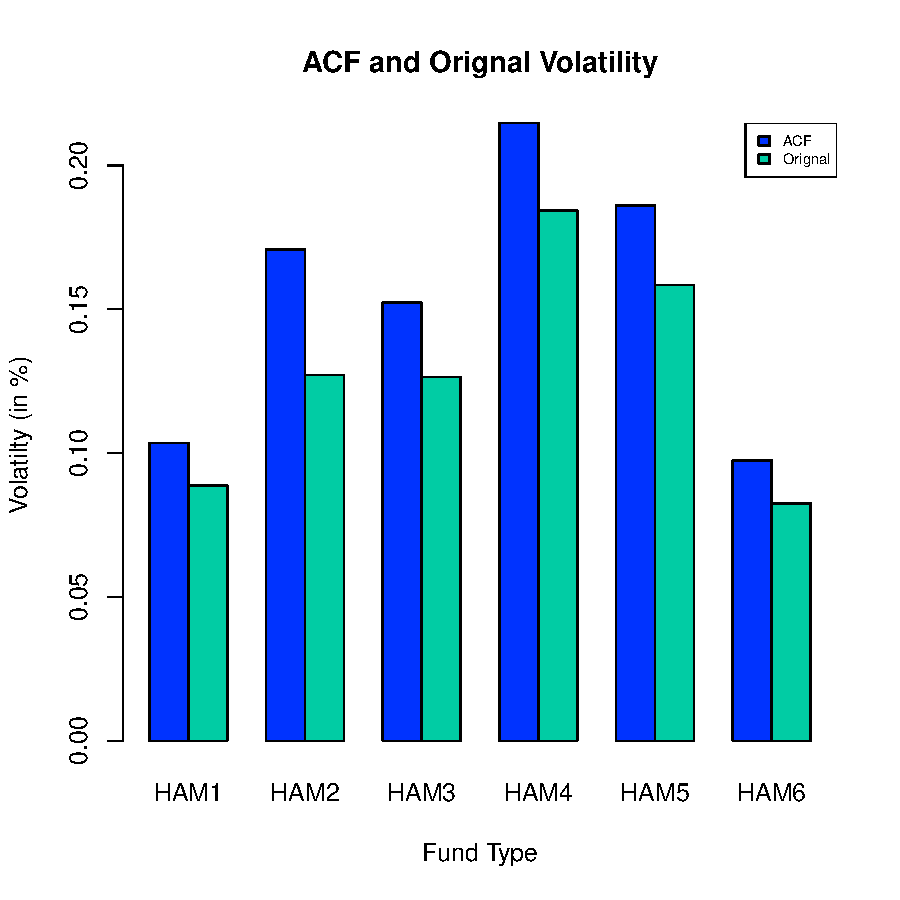
\includegraphics{Managers-005}

From the above figure, we can observe that all the funds, exhibit \textbf{serial auto correlation}, which results in significantly \emph{inflated} standard deviation.
\subsection{Andrew Lo Statistics of Sharpe Ratio}

The building blocks of the \textbf{Sharpe Ratio} : expected returns and volatilities  are unknown quantities that must be estimated statistically and are,
therefore, subject to \emph{estimation error} .To address this question, Andrew Lo derives explicit expressions for the statistical distribution of the Sharpe ratio using
standard asymptotic theory. 

The Sharpe ratio (SR) is simply the return per unit of risk (represented by variability).  In the classic case, the unit of risk is the standard deviation of the returns.
 
\deqn{\frac{\overline{(R_{a}-R_{f})}}{\sqrt{\sigma_{(R_{a}-R_{f})}}}}

The relationship between SR and SR(q) is somewhat more involved for non-
IID returns because the variance of Rt(q) is not just the sum of the variances of component returns but also includes all the co-variances. Specifically, under
the assumption that returns \(R_t\) are stationary,
\begin{equation}
Var[(R_t)] =   \sum_{i=0}^{q-1} \sum_{j=1}^{q-1} Cov(R(t-i),R(t-j)) = q\hat{\sigma^2} + 2\hat{\sigma^2} \sum_{k=1}^{q-1} (q-k)\rho_k \\
\end{equation}

Where  $\rho$\(_k\) = Cov(\(R(t)\),\(R(t-k\)))/Var[\(R_t\)] is the \(k^{th}\) order autocorrelation coefficient's of the series of returns.This yields the following relationship between SR and SR(q):

\begin{equation}
\hat{SR}(q)  =  \eta(q) \\
\end{equation}

Where :

\begin{equation}
\eta(q)  =  \frac{q}{\sqrt{(q\hat{\sigma^2} + 2\hat{\sigma^2} \sum_{k=1}^{q-1} (q-k)\rho_k)}} \\
\end{equation}
 
In given commodity funds, we find results, similar reported in paper, that the annual Sharpe ratio for a hedge fund can be overstated by as much as \textbf{65} \% because of the presence of \textbf{serial correlation}.We can observe that the fund "\textbf{DJUBS.Commodity}", which has the largest drawdown and serial autocorrelation, has it's Andrew Lo Sharpe ratio , \emph{decrease} most significantly as compared to other funds.

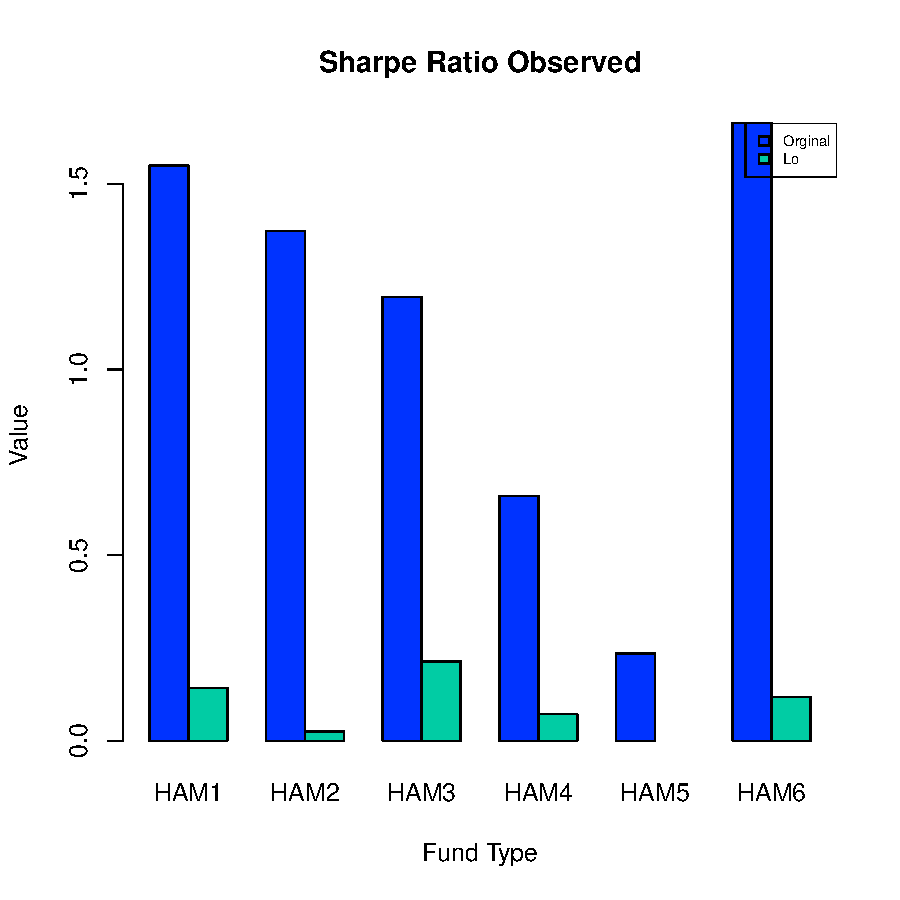
\includegraphics{Managers-006}
\subsection{Conditional Drawdown}
A new one-parameter family of risk measures called Conditional Drawdown (CDD) has
been proposed. These measures of risk are functional of the portfolio drawdown (underwater) curve considered in active portfolio management. For some value of $\hat{\alpha}$ the tolerance parameter, in the case of a single sample path, drawdown functional is defined as the mean of the worst (1 \(-\) $\hat{\alpha}$)100\% drawdowns. The CDD measure generalizes the notion of the drawdown functional to a multi-scenario case and can be considered as a generalization of deviation measure to a dynamic case. The CDD measure includes the Maximal Drawdown and Average Drawdown as its limiting cases.Similar to other cases, \textbf{DJUBS.Commodity}, is the worst performing fund with worst case conditional drawdown greater than \textbf{50\%} and \textbf{Newedge.CTI} performing significantly well among the peer commodity indices with less than \textbf{15\%}.




\subsection{Calmar and Sterling Ratio}
Both the Calmar and the Sterling ratio are the ratio of annualized return over the absolute value of the maximum drawdown of an investment.
{equation}
\begin{equation}
 Calmar Ratio  =  \frac{Return [0,T]}{max Drawdown  [0,T]} \\
\end{equation}

\begin{equation}
 Sterling Ratio  =  \frac{Return [0,T]}{max Drawdown  [0,T] - 10\%} \\
\end{equation}
\begin{Schunk}
\begin{Sinput}
> round(CalmarRatio.Norm(managers[,1:6],1),4)
\end{Sinput}
\begin{Soutput}
                          HAM1   HAM2   HAM3   HAM4    HAM5   HAM6
Normalized Calmar Ratio 0.1744 0.1495 0.1175 0.2493 -0.0048 0.3244
\end{Soutput}
\begin{Sinput}
> round(SterlingRatio.Norm(managers[,1:6],1),4)
\end{Sinput}
\begin{Soutput}
                                           HAM1   HAM2   HAM3  HAM4    HAM5
Normalized Sterling Ratio (Excess = 10%) 0.1052 0.1055 0.0873 0.185 -0.0037
                                           HAM6
Normalized Sterling Ratio (Excess = 10%) 0.1429
\end{Soutput}
\end{Schunk}
For a 1 year \emph{horizon} return, we can see that Newedge.CTI is the clear performer in this metric as well.However, a \textbf{surprising} observed result, is negative \emph{Sterling} and \emph{Calmar} ratio for Morningstar.CLS . 
\subsection{GLM Smooth Index}
GLM Smooth Index is a useful parameter to quantify the degree of autocorrelation.It is a summary statistic for measuring the concentration of autocorrelation present in the lag factors (up-to 6) , which can be defined by the below equation as :
\begin{equation}
\xi =   \sum_{j=0}^{k} \theta _j^2 \\
\end{equation}

This measure is well known in the industrial organization literature as the Herfindahl index, a measure of the concentration of firms in a given industry where $\theta$\(_j\) represents the market share of firm j. Because $\xi_t$\ is confined to the unit interval, and is minimized when all the $\theta$\(_j\) 's are identical, which implies a value of 1/k+1 for $\xi_i$\ ; and is maximized when one coefficient is 1 and the rest are 0. In the context of smoothed returns, a lower value of implies less smoothing, and the upper bound of 1 implies pure smoothing, hence we shall refer to $\theta$\(_j\) as a \textbf{smoothing index}.

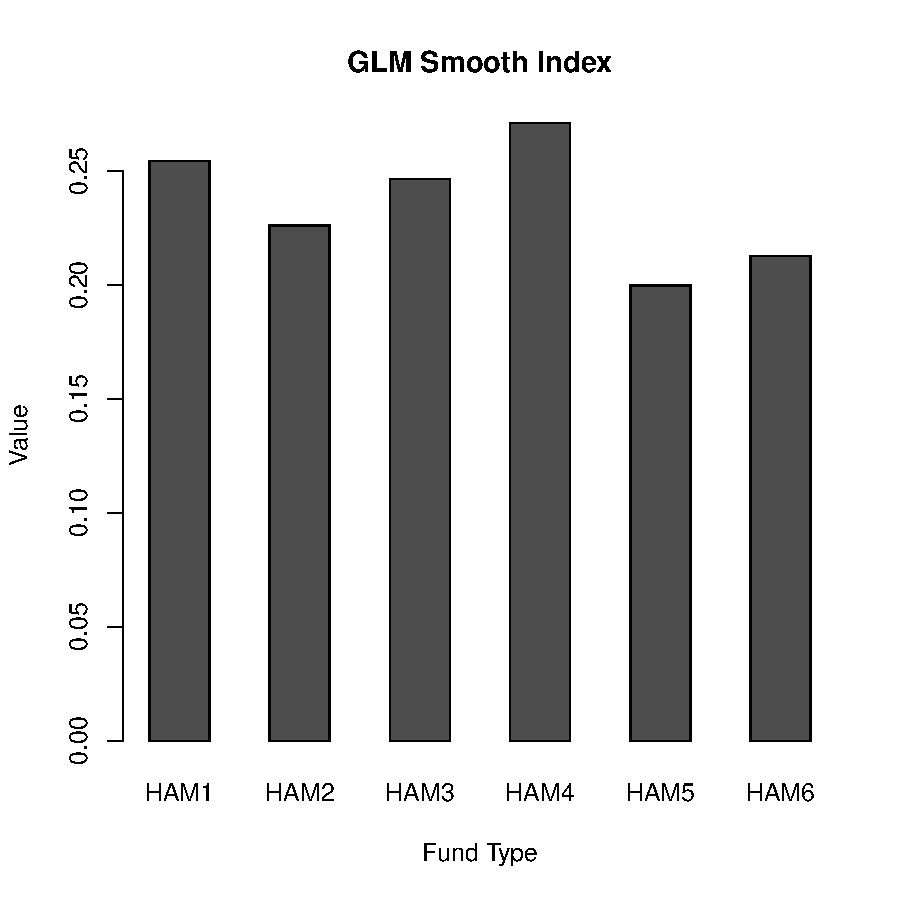
\includegraphics{Managers-008}

For the given chart, we can observe that \textbf{all the funds} have significant level of smooth returns.
\subsection{Acar Shane Maximum Loss}

Measuring risk through extreme losses is a very appealing idea. This is indeed how financial  companies perceive risks. This explains the popularity of loss statistics such as the maximum  drawdown and maximum loss. An empirical application to fund managers performance show that \textbf{very few investments} exhibit  \emph{abnormally high or low drawdowns}. Consequently, it is doubtful that drawdowns statistics can be used 
to significantly distinguish fund managers. This is confirmed by the fact that predicting one-period  ahead drawdown is an almost impossible task. Errors average at the very best 27\% of the true value  observed in the market.

The main concern of this paper is the study of alternative risk measures: namely maximum loss and  maximum drawdown. Unfortunately, there is no analytical formula to establish the maximum drawdown properties under the random walk assumption. We should note first that due to its definition, the maximum drawdown divided by volatility is an only function of the ratio mean divided by volatility.


\begin{equation}
MD / \sigma =  Min \frac{ \sum_{j=1}^{t} X_{j}}{\sigma} = F(\frac{\mu}{\sigma}) \\
\end{equation}

Such a ratio is useful in that this is a complementary statistic to the return divided by volatility ratio. To get some insight on the relationships between maximum drawdown per unit of volatility and mean  return divided by volatility, we have proceeded to Monte-Carlo simulations. We have simulated cash flows over a period of 36 monthly returns and measured maximum drawdown for varied levels of  annualized return divided by volatility varying from minus two to two by step of 0.1. The process has  been repeated six thousand times.

For instance, an investment exhibiting an annualized return/volatility equal to -2 
should experience on average a maximum drawdown equal to six times the annualized volatility. 

Other observations are that: 
\begin{itemize}
\item maximum drawdown is a positive function of the return/volatility ratio 
\item confidence interval widens as the return/volatility ratio decreases  
\end{itemize}

This means that as the return/volatility increases not only the magnitude of drawdown decreases but the confidence interval as well. In others words losses are both smaller and more predictable.

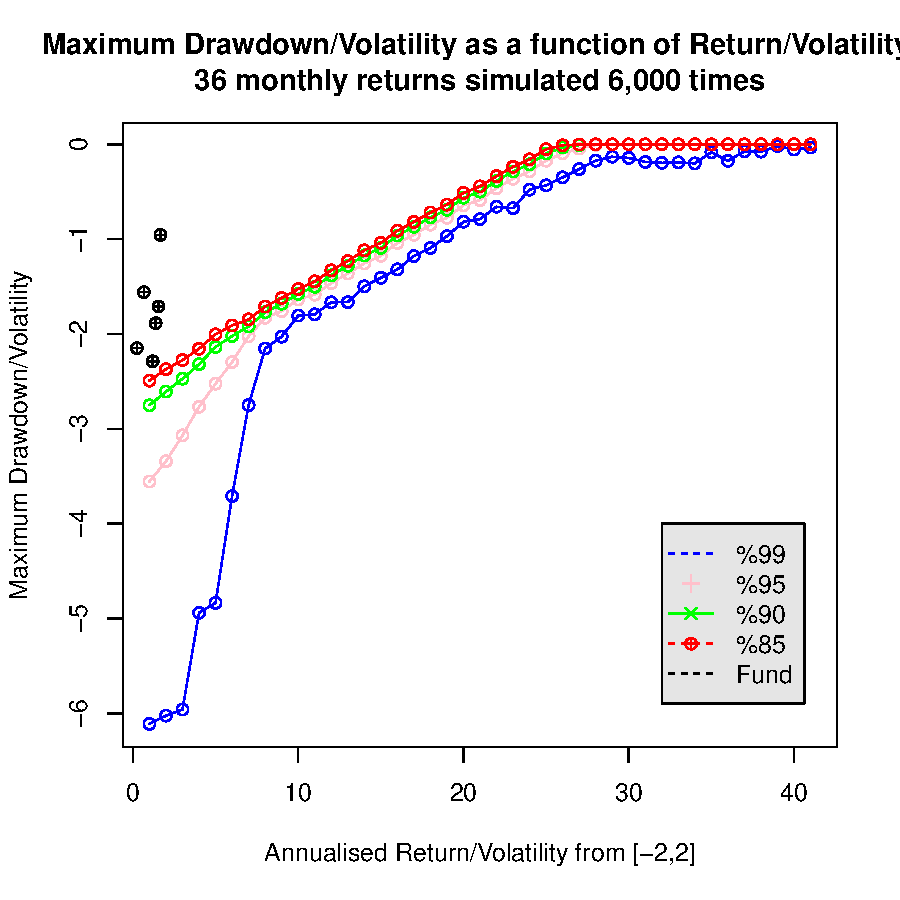
\includegraphics{Managers-009}

As we can see from the \emph{simulated chart}, DJUBS.Commodity comes at the bottom , which imply a \emph{lower} \textbf{return-maximum loss} ratio.

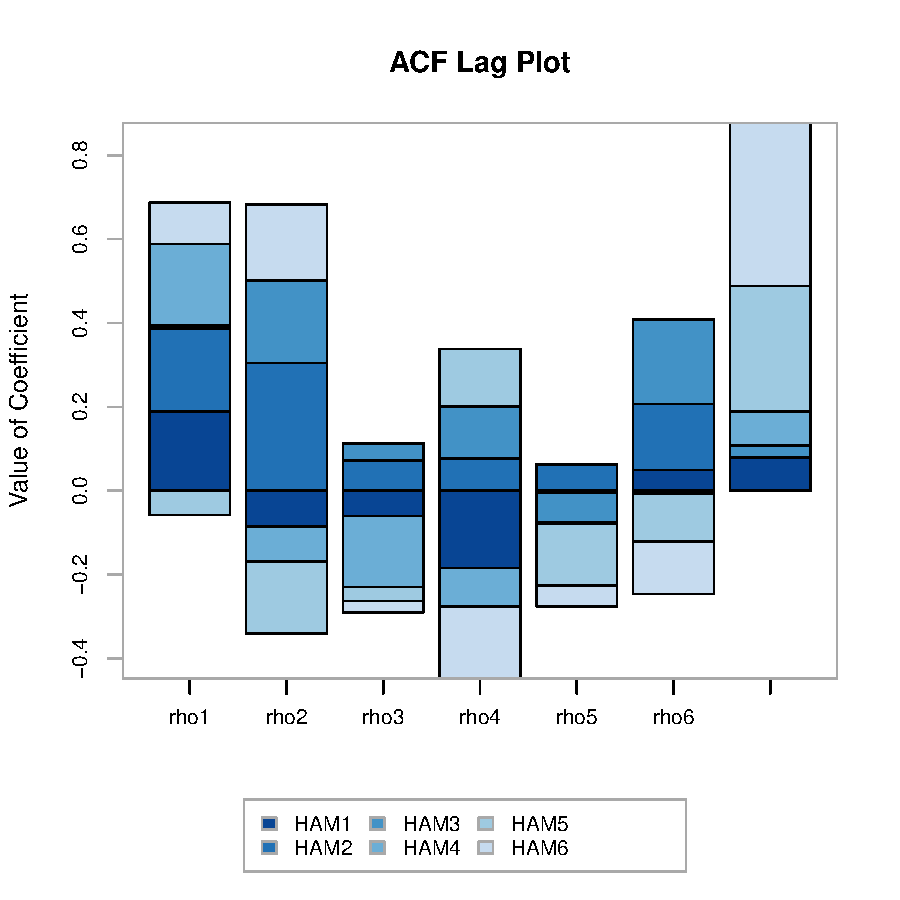
\includegraphics{Managers-010}

Finally, from the autocorrelation lag plot, one can observe, significant \textbf{positive} autocorrelation for \textbf{Newedge.CTI}, which is a \emph{warning} signal in case drawdown occurs, in an otherwise excellent performing fund.
\section{Conclusion}

Analyzing all the function results, one can clearly differentiate \textbf{Newedge.CTI}, as a far superior fund as compared to it's peer.\textbf{MorningStar.CLS}, exhibits highest autocorrelation as well as lowest Calmar/Sterling ratio, but compared on other front, it distinctly outperforms \textbf{DJUBS.Commodity}, which has performed poorly on all the tests. 

The above figure shows the characteristic of the respective fund performance, which is after the period of analysis till \textbf{"July-2013"}.At this moment, we would like the readers, to use the functions developed in the R \textbf{"PerformanceAnalytics"} package, to study ,use it for analysis as well as for forming their own opinion. 

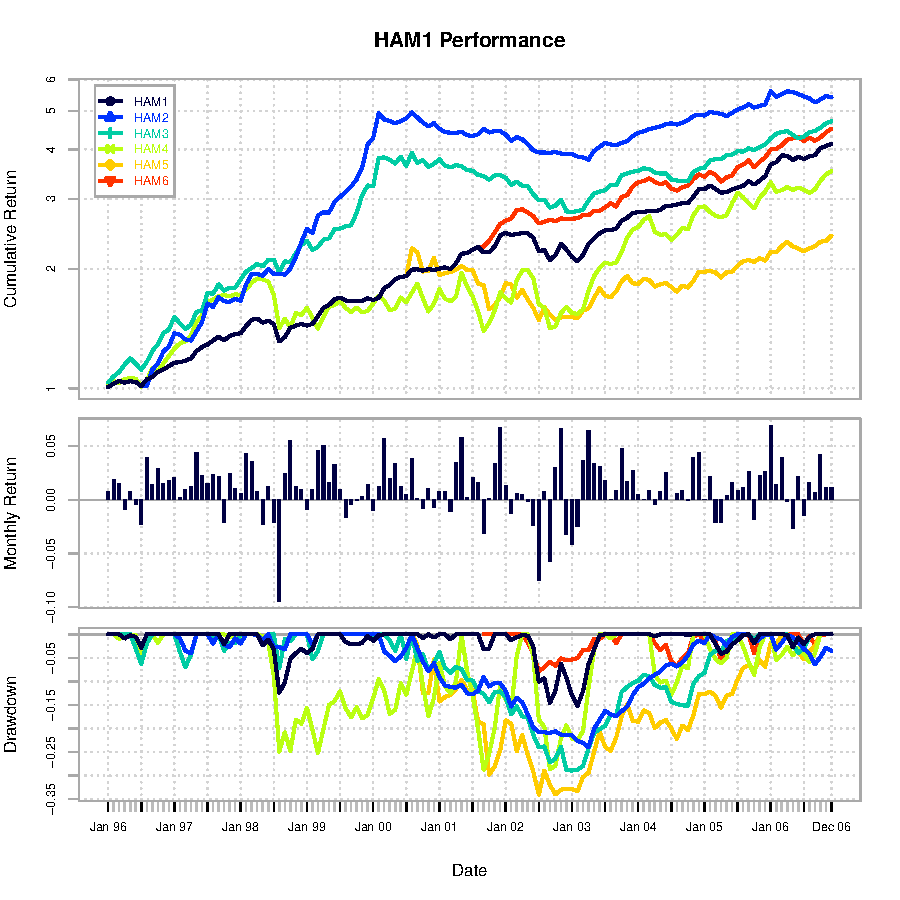
\includegraphics{Managers-011}


\end{document}
